\chapter{Existing technologies}

This chapter gives a short overview of the web application functionality. 
It explores server-side scripting using PHP and client-side scripting using JavaScript in order to obtain observations of user conventions for interaction with web applications.
Afterwards it introduces WASM, followed by an existing project that enables the execution of PHP in a browser.
There is short information about the .NET platform and C\# language.
Blazor and Peachpie are introduced in last sections of this chapter.

\section{PHP}

The basic principle of obtaining a web page is a request-response protocol, where a client sends a request for the web page using an HTTP protocol and receives a response with requested data.
The protocol uses a dedicated message format for communication.
Its typical characteristics is the statelessness, meaning that a server has to retain information about clients and add additional information to the messages in order to distinguish between clients.
\par
Since the server contains the business logic, the browser has to send the necessary data for the required actions via the HTTP message.
The data are usually encoded as a part of \ac{URL} or in the body of the HTTP message.
HTML presents the tag \texttt{<form>} that enables interaction with the web application using a web form.
The figure \ref{img01:php} contains an example of the tag.
The \texttt{<form>} can contain other tags, which are displayed as various types of fields.
The user fills these fields, and the browser sends the data as a new request to the server.
The user can specify how the data are going to be encoded.
The \texttt{GET} method is one of the basic ways.
It encodes the data as a pair of keys and its values to the query part of the URL.
Here is an example of URL
\texttt{http://www.example.com/index.php?par1=hello\&par2=world}.
A query part begins with a question mark.
We can see parameter keys \texttt{par1} and \texttt{par2} containing values \texttt{hello} and \texttt{world}.
Another method is called \texttt{POST} and is encoded in the request body, which does not appear in the URL.
\par
Although PHP \cite{online:phpWiki} was originally designed for user page templating on the server side, it has been adjusted gradually to enable writing the application logic.
PHP is an interpreted language maintained by The PHP Group.
\par
The following language description uses Figure \ref{img01:php} as an example.
The script includes a header, which adds a proper beginning of an HTML document.
Then, it prints a \texttt{POST} content together with a file content whenever the file \texttt{file} was obtained.
There is a form that enables to send an information about the name and attaches a file to the message.
The browser sends the message to the server via \texttt{POST} method when the form is submitted.
The request is handled by \textit{index.php} defined in the \texttt{action}.
In the end, the script includes a proper ending of the document using the \textit{footer.php}.
\par
\begin{figure}
\begin{lstlisting}
<?php
    include("header.php");
?>

<h1>Superglobal POST</h1>
<?php
    foreach($_POST as $key => $value) { ?>
    <p><?php echo $key; ?> => <?php echo $value; ?></p>
<?php } ?>

<h1>File content:</h1>
<p>
<?php 
    if($_FILES["file"])
    {
        echo file_get_contents($_FILES["file"]["tmp_name"]);
    }	
?>
</p>

<form action="/index.php" method="post">
    <label for="name">Name:</label>
    <input type="text" id="name" name="name"><br>
    <label for="file">File:</label>
    <input type="file" id="file" name="file"><br>
    <input type="submit" value="Submit">
</form>

<?php
    inlude("footer.php");
?>
\end{lstlisting}
\caption{An example of PHP code in \textit{index.php} file.}
\label{img01:php}
\end{figure}
\par
As we can see, the PHP code interleaves the HTML code, which has appeared to be a helpful method for data binding.
This HTML interleaving allows inserting a PHP code in \texttt{<?php ... ?>} tag.
These fragments do not have to form individual independent blocks of code closed in curly brackets, as the example demonstrates by using the \texttt{foreach} cycle.
An interpreter executes a script from top to bottom. Everything outside the PHP tag is copied into the body of the request.
\par
We do not see any specification of the type next to the variables.
This is because the type system is dynamic.
A variable represents just a reference to the heap.
Its type is determined during the runtime. 
\par
PHP uses superglobals \cite{online:phpManual}, which are a built-in variables accessible from all scopes of the script.
Following superglobals are relevant for the thesis:
The \texttt{\$\_GET} variable stores parsed query part of the URL.
The \texttt{\$\_POST} variable stores variables which are sent by post method.
The \texttt{\$\_FILES} variable contains information about uploaded files sent by a client.
The uploaded file is saved as a temporary file, and standard reading operations can obtain the content.
This is demonstrated in the previously mentioned example by \texttt{file\_get\_contents} function.
\par
The nature of the request-response semantic usually results in a one-way pass of the application.
After dealing with a request, the script is terminated, meaning that the request is sent, and variables are disposed.
One of the well-known design patterns relating to PHP is the Front controller.
Usually, the main script invokes other parts of the program, based on the request, to deal with it and send the response back.
The idea of this pattern can be shown in Figure \ref{img01:php}.
In the beginning, header rendering is delegated to \textit{header.php} script.
Then, the script renders the body and includes \textit{footer.php}, which cares about the proper ending of the HTML page.
\par
A PHP code can be split by several ways.
Despite the fact that that object-oriented programming is very wide-spread, the most notable characteristics of PHP are global functions.
They are defined in the global scope and accessible from anywhere.
The next option is an object inspired by object-oriented programming.
A PHP script can include a PHP code from other scripts.
They can be recursively included during runtime, where variables remain across the inclusion.
Scripts can be composed into a package, which another code can reuse.

\section{JavaScript}

The client-side code needs to control the rendered page and access a web interface providing additional services, which is usually accessible via JavaScript \cite{online:javascriptWiki} in order to interact with a user.
This section starts with the description of loading JavaScript in a browser.
It introduces a page representation in a browser alongside with page events.
In the end, it presents JavaScript as a scripting language for creating a responsive web page.
\par
We can image a web page structure as a tree.
Its nodes are tags or text fragments, and its edges connect nodes with their children.
Representation of such a tree we can find on \ac{DOM}.
Each node is represented as an object with special parameters relating to HTML and CSS. 
The nodes can contain other nodes representing their children.
Afterwards, there is a document node representing the whole document together with its root node.
\par
The process of generating a web page follows several steps.
The browser parses the HTML page line by line. If a script occurs, the browser starts to execute the code, which can access already parsed tags.
The order of processing is important for the manipulation with HTML structure.
This limitation can be solved by web events mentioned later, but
it is a convention to add scripts to the end of the body part after all HTML tags are parsed.
\par
\begin{figure}[b!]
\begin{lstlisting}
<!DOCTYPE html>
<html>
    <head>
    </head>
    <body>
        <button id="alert">Click to alert</button>
        <script>
            var handler = function (arg) {
                var timer = new Promise((resolve) => {
                    setTimeout(resolve, 1000);
                }); 
        
                timer.then(() => window.alert("Hello world."));
            };  

            var button = window.document.getElementById("alert");
            button.addEventListener("click", handler);
        </script>
    </body>
</html>
\end{lstlisting}
\caption{An example of a JavaScript code.}
\label{img02:javascript}
\end{figure}
\par
Events are the most common method of how to react to a change of a web page state.
Every event can have some handlers (listeners).
Whenever an event occurs, it calls all its listeners.
There are many event types, but we mention the ones that are important for the purpose of this thesis.
HTML tags are the most common entities which can trigger some events.
For example, a button performs an \texttt{onclick} event which is triggered when a client clicks on the button as we can see in Figure \ref{img02:javascript}. 
Other events can represent a state of a page like for example \texttt{onload} which is triggered when the whole HTML document is parsed.
\par
The browser provides more APIs valuable for the application, like fetching extra data from a server or local storage.
These APIs are mentioned as Web API \cite{online:webApi}.
\par
\ac{ES} is a JavaScript standard recommended across browsers.
Later on, the text mentions an abbreviation ES2015 which determines the ECMAScript version.
JavaScript is a high-level language usually executed by a browser's dedicated JavaScript engine.
Browsers run scripts in a sandbox to prevent potential threats of harmful code.
However, it can be also run on a desktop by Node.js, a JavaScript runtime environment running outside the browser.
Figure \ref{img02:javascript} is used to show the language in a simple scenario.
The page contains a button that invokes an alert with a second delay when a client clicks on it.
\par
At first glance, we can see the type system is dynamic, which is similar to PHP.
The \texttt{window} is an essential global variable, which is an object representing the browser window of the running script.
The window object consists of all defined global variables.
It also contains a document property, which is an API for manipulating the DOM tree.
The usage of the document property can be seen in the example, where it is used to get an element by a given id.
JavaScript object is often used as a wrapper of Web APIs.
\par
Functions are first-class citizens in JavaScript.
We can treat them as common variables.
JavaScript supports an event-driven style that helps to react to events conveniently.
There is a handler assigned to the click event in Figure \ref{img02:javascript}.
\par
JavaScript is single-threaded language, but allows an effective synchronous execution.
This can be achieved by \texttt{Promise} object, which is a structure representing an unfinished processes.
Large tasks can be seperated into smaller ones in order to improve the processing time for other parts of the application.
These processes can be chained.
Although the structure can give an illusion of multi-threading, it uses the scheduler for planning the next task executed by the main thread after the previous task is completed or after an event has triggered it.
The single thread is critical for blocking some operations, for example time demanding computatitons which cause thread freezing.
\par
The \texttt{Worker} object represents a web worker \cite{online:workers}, provided by a browser, enabling it to run the script in the background.
The worker limitation is communication with UI thread only by handling message events. 
Messages have to be serialized and deserialized.
\par
JavaScript can organize a code by function and objects similar to PHP.
A module can gather a larger collection of code.
Global entities of the code can be exported to another script.
These exports make an API of the module.
The module advantage is to define the API and to hide the internal code, which is not relevant for the user.

\section{WebAssembly}

WASM \cite{online:wasmConcepts} is a new code format that can be run in current browsers. 
It has a compact byte format, and its performance is near to a native code. 
WASM is designed to be a compiling target of popular low-level languages like C or C++ due to its memory model.
It results in the possibility to run other languages in a browser because its runtime is often written in C or C++.
Browsers enable to run JavaScript alongside WebAssembly, and even more, their codes can call each other.
WASM code has a similar security to a code written in JavaScript because of the usage of the sandbox. 
\par
Thread \cite{online:wasmThreads} support is being discussed nowadays, and it will probably be added in future versions.
After all, new versions of Google Chrome experiments with proper multi-threading support.
As the replacement of using the multi-threading can serve using Web workers, mentioned in JavaScript section.
\par
Despite the support of running WASM in a browser, the browser cannot load it as a standard ES2015 module yet.
WebAssembly JavaScript API was created in order to be able to load a WebAssembly to a browser using JavaScript.

\section{PHP in Browser}

The project PIB \cite{online:pib} aims to use compiled PHP interpreter in WebAssembly, which allows evaluating a PHP code.
The page has to import a specialized module \texttt{php-wasm}. 
A PHP code is evaluated by using JavaScript API or by writing a specialized script block as we can see in Figure \ref{img03:vrzno}.
PHP can afterward interact with JavaScript using a specialized API.
In the figure, the code calls JavaScript \texttt{alert} function with the parameter.
\par
\begin{figure}[H]
\begin{lstlisting}
<script type = "text/php">
	<?php vrzno_run('alert', ['Hello, world!']);
</script>
\end{lstlisting}
\caption{An example of PHP script block executed by the project.}
\label{img03:vrzno}
\end{figure}
\par
At first glance, it might be a good enough approach, but several parts can be problematic due to PHP semantics.
The project does not offer additional support for using PHP scripts on the client side.
For example, superglobals are unused due to a missing server.
This issue is reasonable because this is a server task, but we cannot get information about a query part or handling forms without writing a JavaScript code.
The next problem relates to how a script can navigate to another script without an additional support code, JavaScript.

\section{C\# and .NET 5}

The section introduces the \ac{CLI} \cite{online:cliWiki} before diving into .NET, which is an overused name for several technologies.
CLI is a specification describing executable code and a runtime environment for running it on different architectures.
CLI contains descriptions of a type system, rules, and the virtual machine (runtime environtment), which executes specified \ac{CIL} by translating it to a machine code. 
The virtual machine is named \ac{CLR}.
CIL's advantage is a compilation target of languages like C\#, F\#, and VisualBlasic, which gives us great interoperability.
.NET Framework, .NET 5, and Mono are implementations of CLI.
These implementations are usually uniformly called .NET.
\par
.NET 5 \cite{online:netcoreWiki} is the latest version of .NET Core, which is a cross-platform successor to .NET Framework.
From now on, we refer .NET 5 as .NET, since it should be the only supported framework in the future.
.NET is an open-source project primarily developed by Microsoft.
It consists of runtime environment for executing CIL and many libraries that can represent whole frameworks like is ASP.NET, which aims for web development.
A large collection of code is usually compiled into an assembly containing the code and additional metadata.
An assembly can represent either a library or an executable program.
\par
Mono aims at cross-platform execution of CIL. 
Recently, they started to support compilation \cite{online:monoCompilation} into WebAssembly.
This support allows executing CIL inside browsers.
The compilation has two modes.
The first mode is compilation Mono runtime with using all assemblies.
The second one only compiles Mono runtime, which then can execute .dll files without further compilation of them into WebAssembly.
A consequence of these compilations into WebAssembly is enabling to call JavaScript and WebAPI from C\#.
\par
.NET Standard represents API specifications of .NET libraries across different implementations.
.NET Standard offers to specify minimum requirements for the code.
\par
C\# is a high-level language using strong typing and a garbage collector.
It is a multi-paradigm language, but its common characteristic is the objected-oriented style.
These features cause that C\# is a good language for a huge projects that require discipline from developers and need to keep the code understandable and manageable.

\section{Blazor}

Blazor is a part of the open-source ASP.NET Core framework.
Blazor allows creating client-side web applications written in C\# language.
Blazor framework offers two hosting models \cite{online:hostingModels} that have different approaches to creating web applications. 
The first one is referred to as Blazor Server App and represents a server-side web application using specific communication between a client and a server for better functionality.
This thesis uses the second model, which Microsoft refers to as Blazor WebAssembly App, enabling to move business logic to a client side without using JavaScript.
\par
From now on, the Blazor App is going to be refered as the Blazor WebAssembly App.
The application can be hosted as a standalone project representing a standard ASP.NET Core web server.
The hosting consists of serving application .dlls and static files like HTML, CSS.
The division enables choice of a place for the implementation of business logic.
Thus, the programmer can move the majority of business logic to the client and use the server for connection to a database, or he or she can use the client only for rendering the page.
When we chose the template, there are two main projects to describe.
\par
\begin{figure}\centering
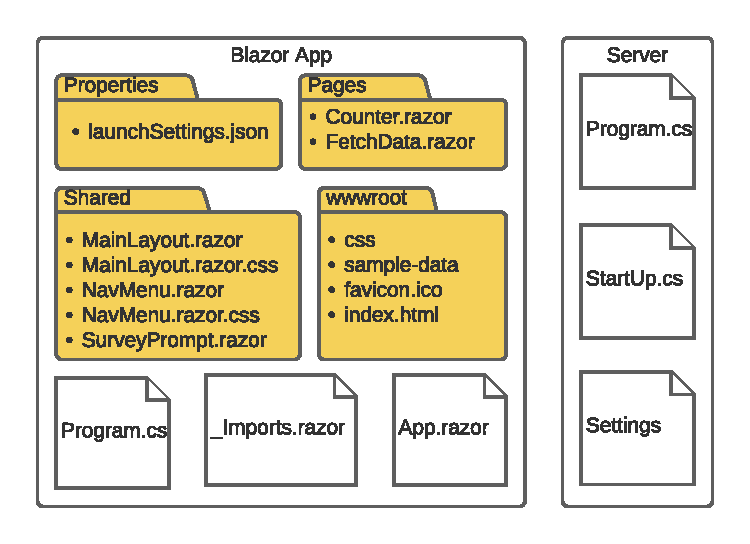
\includegraphics{./img/ProjectStructure}
\caption{Server and WebAssembly App projects.}
\label{img04:projects}
\end{figure} 
\par
As we can see in Figure \ref{img04:projects}, there is a server, which provides the Blazor App to a client.
The project contains a standard builder of a host using a \texttt{StartUp} class, which configures an HTTP request pipeline processing requests in \textit{StartUp.cs} file.
A middleware is a segment of an HTTP request pipeline, which handles some of the functionalities related to request processing.
The pipeline contains a middleware providing the Blazor files.
\par
The structure of the second project (Blazor App) in Figure \ref{img04:projects} is shown to explain basic entities and their interaction with each other.
There are few files with the \texttt{.razor} extension.
Razor is a markup language interleaving HTML with C\#.
Razor uses a special sign \texttt{@} with keywords to identify C\# code in HTML.
Razor compilation results in a pure C\# code representing the web page fragment.
An example of Razor is shown in Figure \ref{img05:razor}.
\par
\begin{figure}
\begin{lstlisting}
@page "/example"
@inject HttpClient Http

<h1>Example</h1>
@if (!loaded)
{
    <p>Loading...</p>
}
else
{
    <p>Ticks: @ticks</p>
}

@code {
    private bool loaded = false;
    private int ticks = 0;

    protected override async Task OnInitializedAsync() {
        ticks = await Http.GetFromJsonAsync<int>("ticks.json");
        loaded = true;
    }
}
\end{lstlisting}
\caption{An example of Razor page.}
\label{img05:razor}
\end{figure}
\par
Although the format can be considered as self-explaining, the keywords are going to be described.
The first line begins with the \texttt{page} keyword determining a part of the URL page.
The next keyword is the \texttt{inject}, representing a \texttt{HttpClient} service injection. 
The \texttt{if} keyword is an control structure iterleaved by an HTML code.
The \texttt{code} keyword contains a regular C\# code, which can be used in the whole \texttt{.razor} file.
\par
A Razor file is compiled into a C\# dedicated class.
The class inherits from \texttt{ComponentBase} or implements \texttt{IComponent}, which provides necessary methods for rendering the page.
Components can be arbitrarily put together in order to form the desired page.
We can see the generated component from Figure \ref{img05:razor} in Figure \ref{img06:component}.
\par
\begin{figure}
\begin{lstlisting}
[Route("/example")]
public class Index : ComponentBase {
    private bool loaded = false;
    private int ticks = 0;
	
    [Inject] private HttpClient Http { get; set; }

    protected override void BuildRenderTree(
    							RenderTreeBuilder __builder) {
        __builder.AddMarkupContent(0, "<h1>Example</h1>");
        if (!loaded)
        {
            __builder.AddMarkupContent(1, "<p>Loading...</p>");
            return;
        }
        __builder.OpenElement(2, "p");
        __builder.AddContent(3, "Ticks: ");
        __builder.AddContent(4, ticks);
        __builder.CloseElement();
    }

    protected override async Task OnInitializedAsync() {
        ticks = await Http.GetFromJsonAsync<int>("ticks.json");
        loaded = true;
    }
}
\end{lstlisting}
\caption{Razor page generated to the C\# class.}
\label{img06:component}
\end{figure}
\par
We can assign the Razor keywords to parts of the code in the figure.
The \texttt{page} keyword stands for the \texttt{Route} attribute.
The \texttt{inject} keyword stands for a class property marked by the \texttt{Inject} attribute.
The parameter is assigned by a dispatcher, during the component initialization.
The \texttt{code} keyword is a part of the class content.
Another markup is transformed into calling a specialized method to the \texttt{BuildRenderTree} function, which describes the page content for rendering.
\par
The component has several stages \cite{online:lifecycle}, which can be used for initialization or action.
Virtual methods of the \texttt{ComponentBase} represent these stages.
We can see the the \texttt{OnInitializedAsync} method, which is invoked after setting the component parameters by the \texttt{SetParameters} method.
The rendering is initiated by calling the \texttt{StateHasChanged} method.
After that, the \texttt{RenderTreeBuilder} is invoked.
When the rendering finishes, Blazor invokes the \texttt{AfterRender} method, which can manipulate with already rendered HTML tags.
\par
Asynchronous processing should be mentioned because it helps with rendering a page containing long-loading content.
Blazor allows using Tasks and async methods, separating the code into smaller tasks planned by a scheduler.
Blocking operations in Blazor are projected into UI because it is single-threaded due to JavaScript and WASM.
\par
Folders \textit{Pages} and \textit{Shared} contain parts of Blazor pages written in Razor.
The \textit{\_Imposts.razor} contains namespaces, which are automatically included in other \texttt{.razor} files.
The next folder is the \textit{wwwroot}, containing static data of the application.
The \textit{index.html}, cares about loading parts of the Blazor application to the browser.
We call all of the static files in the \textit{wwwroot} additional JavaScript scripts and WASM runtime environment Static Web Assets.
\par
The following paragraphs describe the loading of Blazor into the browser to fully understand the interaction between Blazor and the browser.
There is the server, the Blazor App, and other optional user defined projects. 
When the server is started and a client tries to navigate the web application, the following process is done.
The server maps the navigation to \textit{index.html} and sends it back.
\par
\begin{figure}[b!]
\begin{lstlisting}
<body>
    <div id="app">Loading...</div>
    <div id="blazor-error-ui">
        An unhandled error has occurred.
		...
    </div>
    <script src="_framework/blazor.webassembly.js"></script>
</body>

\end{lstlisting}
\caption{\textit{index.html} provided by the server}
\label{img07:index}
\end{figure}
\par 
The \texttt{index.html} contains a script initializing Blazor as we can see in Figure \ref{img07:index}.
The first step is to load all resources, which are defined in a separated file.
Blazor cuts all unnecessary \texttt{.dll} files to reduce the size.
For this reason, all of the \texttt{.dll} files have to be used in the Blazor App code in order to be contained in the file. 
These resources comprise Mono runtime compiled into WASM, additional supporting scripts, and all of the \texttt{.dll} files containing the whole application (Blazor App with referenced libraries).
The supporting scripts initiate the runtime and execute it.
The runtime environment includes the \texttt{.dll} into the application and calls the \texttt{Main} method in the \texttt{Program.cs} defined in Blazor App project.
We can see the process in Figure \ref{img08:wasm}.
\par
\begin{figure}[b!]
\centering
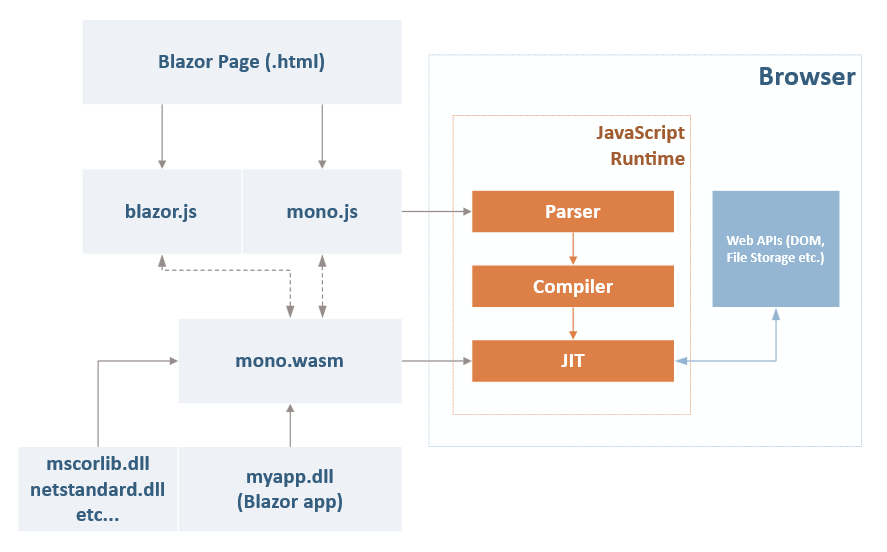
\includegraphics[width=140mm, height=100mm]{./img/BlazorExecution}
\caption{Running a Blazor WebAssembly App on a client side \cite{online:composition}.}
\label{img08:wasm}
\end{figure}
\par
\texttt{Main} method uses the \texttt{WebAssemblyHostBuilder} to set the application.
It defines services, that will be able through the dispatcher.
It sets a root component, which will be rendered as the first.
The host is run.
Afterward, the application provides the dispatcher, cares about rendering, and communicates with the runtime environment to offer interoperability with JavaScript.
\par
The \texttt{App.razor} is the last file for clarification.
It is the root component in default.
It contains a specialized component, the \texttt{Router}, enabling to navigate the pages.
\par
The end of the section describes page navigation \cite{online:routing}, rendering, and handling events.
The navigation can be triggered by an anchor, a form, or by filling up the URL bar.
The URL bar is handled separately by a browser.
JavaScript can influence the remaining elements by adding a listener to their events.
Blazor App handles only an anchor by default.
After clicking on an anchor, a navigation event is fired.
One of the handlers is a JavaScript function, which invokes C\# method through Mono WASM and prevents a browser navigation, when Blazor App handles it. 
The method represents a navigation handler in Blazor App.
The user can add listeners to the handler, but the Router implements default behavior for navigating.
The \texttt{Router} finds all of the components which implement the \texttt{IComponent} interface and tries to render the page according to path matching the \texttt{RouteAttribute} of the component whenever the navigation is triggered.
It creates an instance of the class and fills in its parameters.
The \texttt{Router} calls the \texttt{BuildRenderTree}, which enables running the rendering process.
Previously created intences of the components are disposed.
The navigation can be redirected to the server if there is no match.
\par
The rendering process begins with the \texttt{Renderer} initialized in the application builder.
\texttt{Renderer} keeps a copy of DOM in memory, creates page updates, and calls JavaScript API for changing the web page DOM in a browser, using the runtime interop support.
Blazor provides API for invoking JavaScript functions and vice-versa.
\texttt{Renderer} provides the \texttt{RenderTreeBuilder} for describing page contents.
The builder provides an API for adding various types of content to the \texttt{Batch}, which is a specialized structure for describing previous and present DOM.
Although DOM changes are performance-expensive, a diff algorithm \cite{online:diffAlgorithm} recognizes and tries to reduce the updates in the \texttt{Batch}.
The usage of the \texttt{RenderTreeBuilder} is complicated, because it has to be adapted to the algorithm \cite{online:renderTree}.
The purpose of Razor is to make the usage more effortless when the compilation implements the \texttt{RenderTreeBuilder} for us.
When the \texttt{Renderer} prepares \texttt{Batch}, it calls specialized JavaScript API for changing the page through Mono runtime.
\par
The diff algorithm is used to minimize the browser DOM  update after all components used \texttt{RenderTreeBuilder} to render their content.
This algorithm uses sequence numbers for parts of HTML to identify modified sections.
Sequence numbers are generated in \texttt{RenderTreeBuilder} instructions during a compilation.
The benefit of this information is detecting loops and conditional statements to generating smaller updates of DOM.  
\par
Event handling is just clever usage of the Renderer with dedicated JavaScript API for updating, where the API registers the listener.
When the event is fired, the listener invokes C\# method representing the handler through the WASM runtime.
\par
Blazor brings a new type of library called \ac{RCL}, which differs from normal libraries by the \textit{wwwroot} folder handling \cite{online:rcl}.
During the compilation, Blazor \ac{SDK} generates a configuration file comprising paths to \textit{wwwroot} folders.
The server provides static web assets of these folders to a client by default.
The SDK only involves the folders contained in RCL libraries and WebAssembly projects into the configuration file.

\section{Peachpie}

Peachpie \cite{online:peachpie} is a modern compiler based on Roslyn and Phalanger project.
It allows compiling PHP scripts into a .NET assembly, which can be executed alongside standard .NET libraries.
All information about the scripts are saved in the assembly.
We describe the basics.
\par
Because different languages have a different type system, Peachpie brings dedicated types for representing PHP variables in .NET.
Some of these types are \texttt{PhpValue} representing a standard PHP variable, \texttt{PhpArray}, or \texttt{PhpAlias} which is a reference to \texttt{PhpValue}.
\par
Another abstraction is the \texttt{Context} class.
We can imagine the \texttt{Context} class as a state of the script while it runs.
The \texttt{Context} class consists of superglobals, global variables, declared functions, declared and included scripts.
It also manages input and output, where the resource can be chosen.
The \texttt{Context} class can also be considered as a configuration of the incoming script execution.
All of the information about a request can be arranged to mock every situation on the server-side.
The possibility of saving the \texttt{Context} class and using it later is a significant advantage.
The class provides information about compiled scripts.
\par
Because some PHP extensions are written in C or C++, Peachpie implements them using .NET libraries, which can add additional functions providing an extra nonstandard functionality such as an interaction with a browser.
\par
The main advantage of the compiler is its great interoperability between PHP and .NET.
An option to work with C\# objects, attributes, and calling methods will become crucial for achieving advanced interaction between Blazor and PHP.
\par
The compiler successfully compiled well-known web frameworks like WordPress or Laravel.
Thus many companies use it for combining the existing frameworks with a C\# backend.
\par
At the time of writing this thesis, there are certain limitations emerging from differences between the languages and the stage of Peachpie development.
Availability of PHP extensions depends on binding these functions to C\# code which gives equivalent results. 
The .NET libraries can be executed in an independent environment. 
However, the code can have performance issues in WebAssembly.
The previously mentioned interoperability has limits as well.
C\# constructs like structs and asynchronous methods are undefined in PHP.
